% Created 2021-08-26 Thu 19:04
% Intended LaTeX compiler: pdflatex
\documentclass[presentation,aspectratio=169]{beamer}
\usepackage[utf8]{inputenc}
\usepackage[T1]{fontenc}
\usepackage{graphicx}
\usepackage{grffile}
\usepackage{longtable}
\usepackage{wrapfig}
\usepackage{rotating}
\usepackage[normalem]{ulem}
\usepackage{amsmath}
\usepackage{textcomp}
\usepackage{amssymb}
\usepackage{capt-of}
\usepackage{hyperref}
\usepackage{khpreamble}
\usepackage{amssymb}
\usepgfplotslibrary{groupplots}
\newcommand*{\shift}{\operatorname{q}}
\usetheme{default}
\author{Kjartan Halvorsen}
\date{\today}
\title{Process Automation Laboratory - Modeling second-order systems}
\hypersetup{
 pdfauthor={Kjartan Halvorsen},
 pdftitle={Process Automation Laboratory - Modeling second-order systems},
 pdfkeywords={},
 pdfsubject={},
 pdfcreator={Emacs 26.3 (Org mode 9.4.6)}, 
 pdflang={English}}
\begin{document}

\maketitle

\section{Repetition - Fitting first-order model with delay}
\label{sec:org94daa4d}
\begin{frame}[label={sec:org9cb799e}]{Fitting first-order model with delay}
Assuming a plant model of first-order with time constant \(T\) and delay \(\theta\)
\[  \quad \textcolor{green!50!black}{Y(s)} = \frac{K\mathrm{e}^{-s\theta}}{s\tau + 1}\textcolor{blue!80!black}{U(s)} \quad \overset{U(s) = \frac{u_f}{s}}{\Longrightarrow} \quad \textcolor{green!50!black}{y(t)} = u_f K\big( 1 - \mathrm{e}^{-\frac{t-\theta}{\tau}}\big)u_H(t-\theta)\]
\def\Tcnst{3}
\def\tdelay{0.6}
\def\ggain{2}
\def\uampl{0.8}
\pgfmathsetmacro{\yfinal}{\uampl*\ggain}
\pgfmathsetmacro{\yone}{0.283*\yfinal}
\pgfmathsetmacro{\ytwo}{0.632*\yfinal}
\pgfmathsetmacro{\tone}{\tdelay + \Tcnst/3}
\pgfmathsetmacro{\two}{\tdelay + \Tcnst}

\begin{center}
  \begin{tikzpicture}
    \begin{axis}[
    width=14cm,
    height=4.5cm,
    grid = both,
    xtick = {0, \tdelay, \tone, \two},
    xticklabels = {0, $\theta$, $\theta+\frac{\tau}{3}$, $\theta + \tau$},
    ytick = {0, \yone, \ytwo, \uampl, \yfinal},
    yticklabels = {0, $0.283y_{f}$, $0.632y_f$, $u_f$, $y_f$},
    xmin = -0.2,
    %minor y tick num=9,
    %minor x tick num=9,
    %every major grid/.style={red, opacity=0.5},
    ]
      \addplot [thick, green!50!black, no marks, domain=0:10, samples=100] {\uampl*\ggain*(x>\tdelay)*(1 - exp(-(x-\tdelay)/\Tcnst)} node [coordinate, pos=0.9, pin=-90:{$y(t)$}] {};
      \addplot [const plot, thick, blue!80!black, no marks, domain=-1:10, samples=100] coordinates {(-1,0) (0,0) (0,\uampl) (10,\uampl)} node [coordinate, pos=0.9, pin=-90:{$u(t)$}] {};
    \end{axis}
  \end{tikzpicture}
\end{center}

\[ y_f = \lim_{t\to\infty} y(t) = u_f K \quad \Rightarrow \quad K = \frac{y_f}{u_f}. \]
\end{frame}

\section{Second-order model critically damped}
\label{sec:org05cf766}
\begin{frame}[label={sec:org46667a1}]{Second-order models}
\end{frame}
\begin{frame}[label={sec:org912eb7b}]{Two first-order models in series}
\begin{center}
\begin{tikzpicture}
  \node {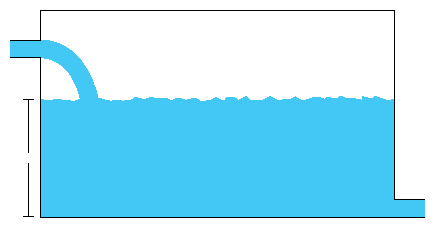
\includegraphics[width=0.4\linewidth]{../../figures/tank-with-hole-no-variables}};
  \node at (5.2,-2.06) {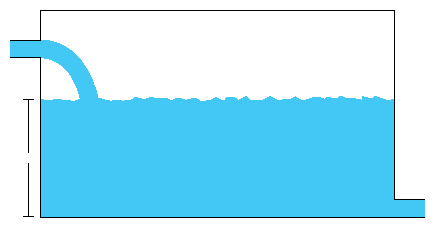
\includegraphics[width=0.4\linewidth]{../../figures/tank-with-hole-no-variables}};
\end{tikzpicture}
\end{center}

\begin{center}
  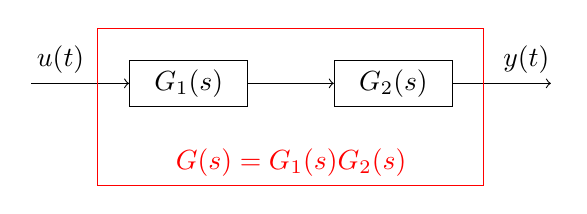
\begin{tikzpicture}[node distance=22mm, block/.style={rectangle, draw, minimum width=15mm}, sumnode/.style={circle, draw, inner sep=2pt}]

    \node[coordinate] (input) {};
    \node[block, right of=input, node distance=20mm] (plant1)  {$G_1(s)$};
    \node[block, right of=plant1, node distance=26mm] (plant2)  {$G_2(s)$};
    \node[coordinate, right of=plant2, node distance=20mm] (output) {};

    \draw[->] (input) -- node[above, pos=0.3] {$u(t)$} (plant1);
    \draw[->] (plant1) -- node[coordinate, ] (mp) { } (plant2);
    \draw[->] (plant2) -- node[above, near end] {$y(t)$} (output);
    \draw[red] (plant1.south west) ++(-4mm,-10mm) rectangle ++(49mm, 20mm);

    \node[red,below of=mp, node distance=10mm] {$G(s) = G_1(s)G_2(s)$};
  \end{tikzpicture}
\end{center}
\end{frame}



\begin{frame}[label={sec:orgeaac7ac}]{Fitting second-order critically-damped model}
\alert{Model with two identical time-constants.}
Assuming model 
\[ \textcolor{green!50!black}{Y(s)} = \frac{K}{(s\tau + 1)^2}\textcolor{blue!80!black}{U(s)} \quad \overset{U(s) = \frac{u_f}{s}}{\Longrightarrow} \quad \textcolor{green!50!black}{y(t)} = u_f K\Big( 1 - (1+\frac{t}{\tau}\big)\mathrm{e}^{-\frac{t}{\tau}}\Big)u_H(t)\]
\def\Tcnst{2}
\def\tdelay{0.0}
\def\ggain{2}
\def\uampl{0.8}
\pgfmathsetmacro{\yfinal}{\uampl*\ggain}
\pgfmathsetmacro{\ytwo}{\yfinal*(1-2*exp(-1))}
\pgfmathsetmacro{\two}{\tdelay + \Tcnst}

\begin{center}
  \begin{tikzpicture}
    \begin{axis}[
    width=14cm,
    height=4.5cm,
    grid = both,
    xtick = {0, \two},
    xticklabels = {0,  $\tau$},
    ytick = {0, \ytwo, \uampl, \yfinal},
    yticklabels = {0, $ $, $u_f$, $y_f$},
    xmin = -0.2,
    clip = false,
    %minor y tick num=9,
    %minor x tick num=9,
    %every major grid/.style={red, opacity=0.5},
    ]
      \addplot [thick, green!50!black, no marks, domain=0:11, samples=100] {\uampl*\ggain*(x>\tdelay)*(1 - (1+x/\Tcnst)*exp(-(x-\tdelay)/\Tcnst)} node [coordinate, pos=0.9, pin=-90:{$y(t)$}] {};
      \addplot [const plot, thick, blue!80!black, no marks, domain=-1:11, samples=100] coordinates {(-1,0) (0,0) (0,\uampl) (11,\uampl)} node [coordinate, pos=0.9, pin=-90:{$u(t)$}] {};
      \node at (axis cs: 11, -0.3) {$t$};
    \end{axis}
  \end{tikzpicture}
\end{center}

\alert{Individual activity} Evaluate the response \(y(t)\) at the time instants \(t=\tau\)!
\end{frame}


\begin{frame}[label={sec:org8ae4797}]{Fitting second-order critically-damped model}
\alert{Model with two identical time-constants.}
Assuming model 
\[ \textcolor{green!50!black}{Y(s)} = \frac{K}{(s\tau + 1)^2}\textcolor{blue!80!black}{U(s)} \quad \overset{U(s) = \frac{u_f}{s}}{\Longrightarrow} \quad \textcolor{green!50!black}{y(t)} = u_f K\Big( 1 - (1+\frac{t}{\tau}\big)\mathrm{e}^{-\frac{t}{\tau}}\Big)u_H(t)\]
\def\Tcnst{2}
\def\tdelay{0.0}
\def\ggain{2}
\def\uampl{0.8}
\pgfmathsetmacro{\yfinal}{\uampl*\ggain}
\pgfmathsetmacro{\ytwo}{\yfinal*(1-2*exp(-1))}
\pgfmathsetmacro{\ytwofactor}{(1-2*exp(-1))}
\pgfmathsetmacro{\two}{\tdelay + \Tcnst}

\begin{center}
  \begin{tikzpicture}
    \begin{axis}[
    width=14cm,
    height=4.5cm,
    grid = both,
    xtick = {0, \two},
    xticklabels = {0,  $\tau$},
    ytick = {0, \ytwo, \uampl, \yfinal},
    yticklabels = {0, $\ytwofactor y_f$, $u_f$, $y_f$},
    xmin = -0.2,
    clip = false,
    %minor y tick num=9,
    %minor x tick num=9,
    %every major grid/.style={red, opacity=0.5},
    ]
      \addplot [thick, green!50!black, no marks, domain=0:11, samples=100] {\uampl*\ggain*(x>\tdelay)*(1 - (1+x/\Tcnst)*exp(-(x-\tdelay)/\Tcnst)} node [coordinate, pos=0.9, pin=-90:{$y(t)$}] {};
      \addplot [const plot, thick, blue!80!black, no marks, domain=-1:11, samples=100] coordinates {(-1,0) (0,0) (0,\uampl) (11,\uampl)} node [coordinate, pos=0.9, pin=-90:{$u(t)$}] {};
      \node at (axis cs: 11, -0.3) {$t$};
    \end{axis}
  \end{tikzpicture}
\end{center}

\[ y_f = \lim_{t\to\infty} y(t) = u_f K \quad \Rightarrow \quad K = \frac{y_f}{u_f}. \]
\end{frame}

\section{Second-order model under-damped}
\label{sec:orge4875a1}

\begin{frame}[label={sec:org4913578}]{Second-order under-damped models}
A system with ODE
$$ \ddot{y} + 2\zeta\omega_n\dot{y} + \omega_n^2 y = \omega_n^2 u, $$
becomes in the Laplace domain
$$ Y(s) = \frac{\omega_n^2}{s^2 + 2\zeta\omega_n s + \omega_n^2} U(s). $$
\begin{columns}
\begin{column}{0.4\columnwidth}
\begin{itemize}
\item \alert{\(\zeta\)} is called the \emph{damping ratio}.
\item \alert{\(\omega_n\)} is called the \emph{natural frequency} (of the system).
\end{itemize}
\end{column}

\begin{column}{0.6\columnwidth}
\begin{center}
    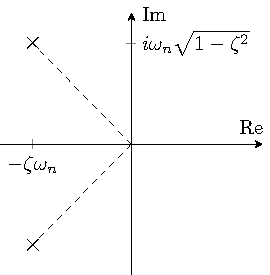
\includegraphics[width=4cm]{../../figures/implane-second-order-poles}
\end{center}
\end{column}
\end{columns}
\end{frame}

\begin{frame}[label={sec:orgaf0b169}]{Second-order under-damped models}
$$ Y(s) = \frac{\omega_n^2}{s^2 + 2\zeta\omega_n s + \omega_n^2} U(s), \qquad \overset{U(s) = \frac{u_f}{s}}{\Longrightarrow} $$
$$     y(t) = 1 - \frac{\mathrm{e}^{-\zeta\omega_nt}}{\sqrt{1-\zeta^2}} \sin\big( \sqrt{1-\zeta^2}\omega_n t + \phi \big) $$


\begin{columns}
\begin{column}{0.3\columnwidth}
\begin{center}
    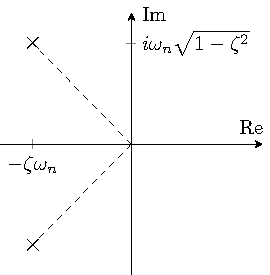
\includegraphics[width=4cm]{../../figures/implane-second-order-poles}
\end{center}
\end{column}

\begin{column}{0.7\columnwidth}
\begin{center}
    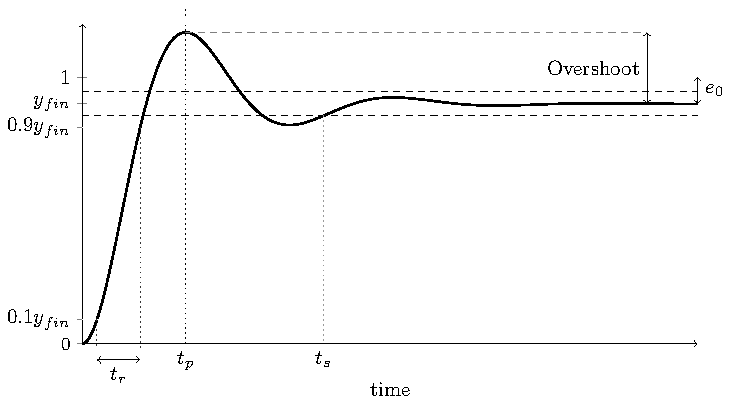
\includegraphics[width=8cm]{../../figures/step-response-specifications}
\end{center}
\end{column}
\end{columns}
\end{frame}

\begin{frame}[label={sec:org303851d}]{Second-order under-damped models}
\begin{columns}
\begin{column}{0.3\columnwidth}
\begin{center}
    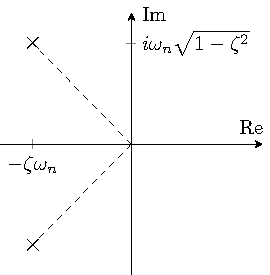
\includegraphics[width=4cm]{../../figures/implane-second-order-poles}
\end{center}

\[    t_r \approx \frac{\pi}{2\omega_n}, \qquad   t_s \approx \frac{4}{\zeta\omega_n}, \]
\end{column}
\begin{column}{0.7\columnwidth}
\begin{center}
    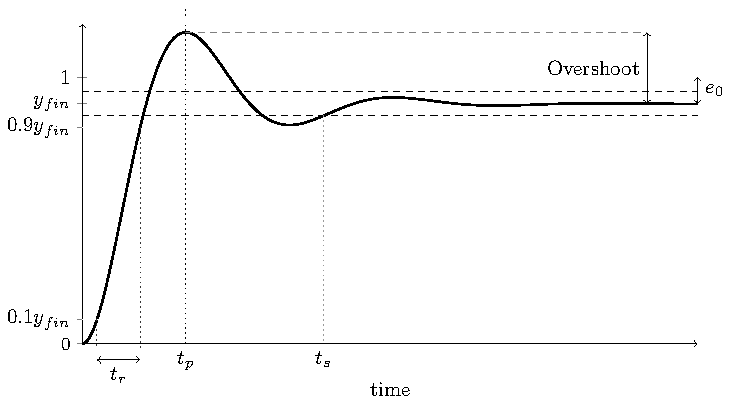
\includegraphics[width=8cm]{../../figures/step-response-specifications}
\end{center}

\[    t_p \approx \frac{\pi}{\sqrt{1 - \zeta^2}\omega_n}, \qquad    \zeta \approx \sqrt{\frac{(\ln \frac{PO}{100})^2}{\pi^2 + (\ln \frac{PO}{100})^2}} \]
\end{column}
\end{columns}
\end{frame}

\begin{frame}[label={sec:org2b00872}]{Second-order under-damped models}
\alert{Activity in pairs} Determine the poles of the system!
\begin{columns}
\begin{column}{0.3\columnwidth}
\begin{center}
    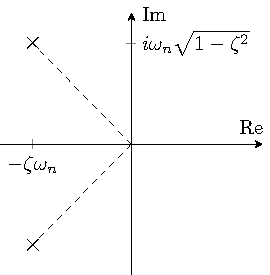
\includegraphics[width=4cm]{../../figures/implane-second-order-poles}
\end{center}

\[    t_s \approx \frac{4}{\zeta\omega_n}, \]
\end{column}
\begin{column}{0.7\columnwidth}
\begin{center}
\begin{tikzpicture}
   \node[anchor=south west] {    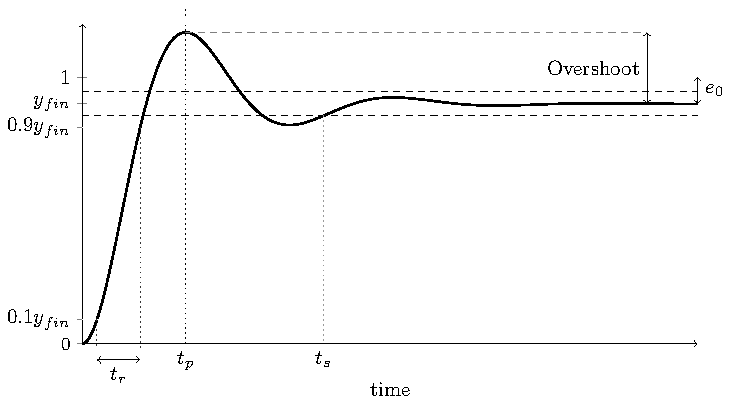
\includegraphics[width=8cm]{../../figures/step-response-specifications}};
   \draw[red] (2.2,4.2) -- ++(-1.2,0) node[left] {$1.3 y_f$};
   \draw[red, dotted] (3.7,0.8) -- ++(0,-0.3) node[below] {$2$};

\end{tikzpicture}
\end{center}

\[   \zeta \approx \sqrt{\frac{(\ln \frac{PO}{100})^2}{\pi^2 + (\ln \frac{PO}{100})^2}} \]
\end{column}
\end{columns}
\end{frame}
\end{document}